\documentclass[a4paper,10pt,leqno]{article} 
\usepackage[utf8]{inputenc}
\usepackage[a4paper]{geometry}
\usepackage[magyar]{babel}
\usepackage{amsmath}
\usepackage{amssymb}
\usepackage{pgf, tikz}
\frenchspacing 
\pagestyle{empty}
\newcommand{\ki}[2]{\hfill {\it #1 (#2)}\medskip}
\newcommand{\vonal}{\hbox to \hsize{\hskip2truecm\hrulefill\hskip2truecm}}
\newcommand{\degre}{\ensuremath{^\circ}}
\newcommand{\tg}{\mathop{\mathrm{tg}}\nolimits}
\newcommand{\ctg}{\mathop{\mathrm{ctg}}\nolimits}
\newcommand{\arc}{\mathop{\mathrm{arc}}\nolimits}
\begin{document}
\begin{center} \Large {\em 24. Nemzetközi Magyar Matematika Verseny} \end{center}
\begin{center} \large{\em Szabadka, 2015. április 8-12.} \end{center}
\smallskip
\begin{center} \large{\bf 10. osztály} \end{center}
\bigskip 

{\bf 1. feladat: } A XXIV. Nemzetközi Magyar Matematika Verseny tiszteletére Frici rajzolt Szabadka főterére egy 24 oldalú szabályos sokszöget. Hány olyan egyenlő szárú háromszöget rajzolhatna, amelynek minden csúcsa ennek a sokszögnek egy csúcsa, és minden oldala ennek a sokszögnek egy átlója?

\ki{Erdős Gábor}{Nagykanizsa, Magyarország}\medskip

{\bf Megoldás: } Rögzítsük az egyik csúcsot, legyen ez a szárak metszéspontja. Számozzuk meg a csúcsokat úgy, hogy ez legyen az 1-es, a számozás pedig az óramutató járásának megfelelő irányban folyamatos. A szomszédos csúcsok nem lehetnek a háromszög alapjai, mert akkor a háromszög 2 oldala nem átló lesz, hanem oldal. De minden, az 1-es csúcsból induló átlóra merőleges átló igen. Ilyenek: 3-ból a 23-ba, 4-ből a 22-be, 5-ből a 21-be, \ldots, 12-ből a 14-be. Ilyen átlóból 10 darab van. Ugyanez elmondható minden csúcsra, így kapunk $24\cdot 10=240$ háromszöget. Mit számoltunk többször? A szabályos háromszögeket, azokat mindhárom csúcsuknál megszámoltuk. Mivel ilyen háromszögből 8 darab van (pl. az előbbi számozás szerint az 1, 9, 17 csúcsok által alkotott háromszög, illetve ennek elforgatottjai), így ezeket háromszor számoltuk, tehát kétszer ki kell vonni őket. A megfelelő háromszögek száma tehát $240-2\cdot 8=224$.


\vonal

{\bf 2. feladat: } Ha $x,y,z\in[-3, 5]$, akkor igazold, hogy
$$\sqrt{5x-3y-xy+15}+
\sqrt{5y-3z-yz+15}+\sqrt{5z-3x-xz+15}\le 12.$$
Mikor állhat fenn az egyenlőség?

\ki{Kovács Béla}{Szatmárnémeti, Erdély}\medskip

{\bf Megoldás: } A gyökjelek alatti kifejezések szorzattá alakíthatók:
$$\sqrt{(x+3)(5-y)}+
\sqrt{(y+3)(5-z)}+\sqrt{(z+3)(5-x)}\le 12.$$
A feladat feltétele miatt az $x, y, z$ valós számokra teljesül, 
hogy $x+3\ge 0$, 
$5-x\ge 0$, 
$y+3\ge 0$, 
$5-y\ge 0$,  
$z+3\ge 0$
és 
$5-z\ge 0$, tehát a gyökös kifejezések értelmezettek.

Alkalmazzuk mindegyik gyökös kifejezésre a számtani és mértani középarányosok közötti összefüggést. Ekkor
\begin{align*}
\sqrt{(x+3)(5-y)}\le\frac{x+3+5-y}{2},\\
\sqrt{(y+3)(5-z)}\le\frac{y+3+5-z}{2},\\
\sqrt{(z+3)(5-x)}\le\frac{z+3+5-x}{2}.
\end{align*}
Összeadva a fenti egyenlőtlenségeket megkapjuk a bizonyítandó egyenlőtlenséget, azaz
\begin{align*}
~&\sqrt{(x+3)(5-y)}+
\sqrt{(y+3)(5-z)}+
\sqrt{(z+3)(5-x)}\le\\
~&\le\frac{x+3+5-y}{2}+
\frac{y+3+5-z}{2}+
\frac{z+3+5-x}{2}=\frac{24}{2}=12.
\end{align*}
Egyenlőség akkor áll fenn, ha a zárójeleken belül levő kifejezések megegyeznek, azaz 
ha $x+3=5-y$, $y+3=5-z$ és $z+3=5-x$, ez pedig az  $x=y=z=1$ eset. 

\vonal


{\bf 3. feladat: } Hány olyan egyenlőszárú trapéz létezik, amelynek a kerülete 2015 és az oldalak mérőszáma egész szám?

\ki{Szabó Magda}{Szabadka, Vajdaság}\medskip

{\bf 1. megoldás: } Legyenek az oldalak rendre $a, c, b, c$, ahol $a, b, c\in\mathbb{Z}^+$ és legyen $a>b$. Ekkor érvényes az $a<c+b+c$ egyenlőtlenség és a feladat feltétele alapján
$$a<\frac{a+b+2c}{2}=\frac{2015}{2}.$$
Az $a$ valamely rögzített értékére az $\{1, 2, 3,\ldots, 1007\}$ halmazból a $b$ értéke bármely $a$-nál kisebb érték lehet, de paritásban különbözőek kell hogy legyenek. Ennek alapján a lehetőségek száma $\left[\dfrac{a}{2}\right]$, ekkor a $c$ értéke egyértelmű és a trapéz is egyértelműen meghatározott az oldalaival. A trapézok keresett száma:
$$\sum_{a=1}^{1007}\left[\frac{a}{2}\right]=
0+1+1+2+2+\ldots+502+502+503+503=
2\cdot\frac{504\cdot 503}{2}=253512.$$

{\bf 2. megoldás: } Jelölje $a$ a trapéz rövidebb alapját, $c$ a szárakat, a hosszabb alap pedig az ábra alapján legyen
$$b+a+b=a+2b.$$
 Ekkor $2a+2b+2c=2015$, ahonnan
$$a+b+c=1007{,}5.$$
Mivel $b<c$ és $a,c\in \mathbb{Z}^+$, vehetjük, hogy
$$b=d-0{,}5, \text{~ahol~} d\in\mathbb{Z}^+.$$
Most teljesül, hogy 
$a+c+d=1008$ és $a\ge 1$, ahonnan $c+d\le 1007$.
A feladat feltételeivel ekkor ekvivalens az, hogy 
$d\le c$, $c, d\in\mathbb{Z}^+$ és $c+d\le 1007$. 
Mivel $2d\le c+d\le 1007$, így $d\le 503$. 
Ha $d\in\{1, 2, 3,\ldots, 503\}$, akkor 
$c\in\{d, d+1,\ldots,1007-d\}$.
A trapézok keresett száma tehát
$$\sum_{d=1}^{503}(1007-d-d+1)=
\sum_{d=1}^{503}(1008-2d)=
503\cdot 1008-2\cdot\frac{503\cdot 504}{2}=
503\cdot 504=253512.$$

\begin{center}
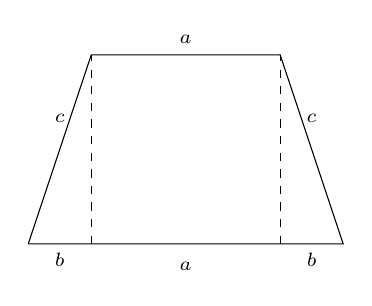
\begin{tikzpicture}[x=0.4cm, y=0.4cm]
\draw(0,0)--(10,0)--(8,6)--(2,6)--(0,0);
\draw[dashed] (2,0) -- (2,6);
\draw[dashed] (8,0) -- (8,6);
\begin{scriptsize}
\draw (1,-0.5) node {$b$};
\draw (9,-0.5) node {$b$};
\draw (5,-0.7) node {$a$};
\draw (5,6.5) node {$a$};
\draw (1,4) node {$c$};
\draw (9,4) node {$c$};
\end{scriptsize}
\end{tikzpicture}
\end{center}

\vonal


{\bf 4. feladat: } Határozd meg mindazokat az $a$ valós számokat, melyekre az 
$$ax^2+(1-a^2)x-a>0$$
egyenlőtlenség egyetlen $x$ megoldására sem igaz, hogy $|x|>2$.

\ki{Csikós Pajor Gizella}{Szabadka, Vajdaság}\medskip

{\bf Megoldás: } Ha egyetlen $x$ megoldásra sem igaz, hogy $|x|>2$, akkor minden $x$ megoldásra igaz, hogy $|x|\le 2$ vagyis, hogy $-2\le x \le 2$.
Az $ax^2+(1-a^2)x-a=0$ egyenlet $a\ne 0$ esetén másodfokú, és gyökei az $x_{1/2}=\dfrac{-1+a^2\pm(1+a^2)}{2a}$ számok, ahonnan $x_1=-\dfrac{1}{a}$ és $x_2=a$.
 
\begin{enumerate}
\item Ha $a=0$, akkor az $x>0$ egyenlőtlenséget kapjuk, amely halmazban van olyan $x$ amelyre $|x|>2$, így $a\ne 0$.  

\item Ha $a>0$, akkor a megfelelő parabolának minimuma van (felfelé nyíló) és akkor pozitív, amikor $x<-\dfrac{1}{a}$ vagy $x>a$. Mivel bármely $a>0$  esetén található olyan $x$ a megoldáshalmazból, amelyre $|x|>2$, így $a>0$ sem lehetséges.

\item Ha $a<0$, akkor a megfelelő parabolának maximuma van (lefelé nyíló) és akkor pozitív, amikor $a<x<-\dfrac{1}{a}$. Ha az $a<x<-\dfrac{1}{a}$ feltétel mellett $-2\le x \le 2$ is érvényes, akkor $a\ge -2$ és $-\dfrac{1}{a}\le 2$, illetve $a\le -\dfrac{1}{2}$ kell, hogy teljesüljön. 
\end{enumerate}

Ezek szerint a keresett $a$ számokra a $-2\le a \le -\dfrac{1}{2}$ feltétel kell hogy teljesüljön.


\vonal


{\bf 5. feladat: } Oldd meg a következő egyenletet a valós számok halmazán:
$$\left|2x-57-2\cdot\sqrt{x-55}+\frac{1}{x-54-2\cdot\sqrt{x-55}}\right|=|1-x|.$$

\ki{Bíró Bálint}{Eger, Magyarország}\medskip

{\bf Megoldás: } A négyzetgyökös kifejezés akkor értelmezett, ha $x\ge 55$. Először az egyenletet a következő alakra hozzuk:
$$\left|x-55-2\cdot\sqrt{x-55}+\frac{1}{x-54-2\cdot\sqrt{x-55}}+x-3\right|=|1-x|.$$
Vezessük be az $x-54-2\cdot\sqrt{x-55}=a$ helyettesítést. Az egyenletben szereplő tört nevezője miatt nyilvánvaló, hogy $a\ne 0$. Könnyen belátható, hogy 
$$a=\left(1-\sqrt{x-55}\right)^2,$$
ez pedig azt jelenti, hogy csak $a>0$ állhat fenn.
Ezzel a jelöléssel az eredeti egyenlet:
$$\left|a+\frac{1}{a}+x-3\right|=|1-x|$$
alakba írható, amelyből két lehetséges esetet írhatunk fel:
\begin{equation}
a+\frac{1}{a}+x-3=1-x, \tag{A}
\end{equation}
vagy
\begin{equation}
a+\frac{1}{a}+x-3=x-1. \tag{B}
\end{equation}
Az (A) egyenletből $a+\dfrac{1}{a}=4-2x$ következik, ez azonban az $x\ge 55$ és az $a>0$ feltételek mellett nem teljesülhet, hiszen az egyenlet két oldalának előjele eltérő. Ezért az (A) egyenletnek nincs megoldása.

A (B) egyenletből azt kapjuk, hogy $a+\dfrac{1}{a}=2$. Ismeretes a pozitív számokra vonatkozó  $a+\dfrac{1}{a}\ge 2$ nevezetes egyenlőtlenség, amelyben az egyenlőség pontosan akkor teljesül, ha $a=1$.
 
Az $a=\left(1-\sqrt{x-55}\right)^2$ összefüggés szerint tehát: $\left(1-\sqrt{x-55}\right)^2=1$.
Ez az egyenlőség ismét kétféleképpen lehetséges:
\begin{equation}
1-\sqrt{x-55}=1, \tag{C}
\end{equation}
vagy
\begin{equation}
1-\sqrt{x-55}=-1. \tag{D}
\end{equation}
A (C) egyenlet megoldása $x=55$, a (D) egyenlet megoldása pedig $x=59$.
Egyszerű számolással ellenőrizhető, hogy ezek a számok valóban kielégítik az eredeti egyenletet, ezért a feladat megoldáshalmaza $M=\{55, 59\}$.

\vonal


{\bf 6. feladat: } Egy konvex négyszöget átlói négy háromszögre bontanak. Ha mind a négy háromszög területének a mértéke egész szám, akkor végződhet-e 2015-re a négy terület mértékének szorzata? Lehet-e ez a szorzat olyan egész szám, amelynek utolsó négy jegye 2015, azaz lehet-e 
$t_1\cdot t_2\cdot t_3 \cdot t_4 = \overline{\ldots2015}$, ha $t_1, t_2, t_3, t_4$ jelöli a háromszögek területeinek mértékét?

\ki{Katz Sándor}{Bonyhád, Magyarország}\medskip

{\bf Megoldás: } Legyenek a négyszög csúcsai $A, B, C, D$, az átlók metszéspontja pedig $E$. Az átlók behúzásával keletkezett négy háromszög területe legyen $t_1$, $t_2$, $t_3$ és $t_4$.
Az $ABE$ és $AED$ háromszögek magassága ugyanaz, ezért területeik aránya $t_1:t_4=BE:ED$. Ugyanígy a  $CBE$ és $CED$ háromszögekre megkapható, hogy $t_2:t_3=BE:ED$. A két egyenlőségből $t_1\cdot t_3=t_2\cdot t_4$ adódik.
(\textit{Ezzel beláttuk, hogy egy konvex négyszög átlói által meghatározott négy háromszög területe közül két-két szemközti szorzata egyenlő.})
Eszerint a négy háromszög területének szorzata: $t_1\cdot t_2\cdot t_3\cdot t_4=(t_1\cdot t_3)^2$.

\begin{center}
\definecolor{uuuuuu}{rgb}{0.26666666666666666,0.26666666666666666,0.26666666666666666}
\begin{tikzpicture}[line cap=round,line join=round,x=0.8cm,y=0.8cm]
\clip(-3.06,1.08) rectangle (1.7,4.76);
\draw (-2.38,1.44)-- (1.26,1.5);
\draw (1.26,1.5)-- (0.54,4.36);
\draw (0.54,4.36)-- (-2.28,3.84);
\draw (-2.28,3.84)-- (-2.38,1.44);
\draw (0.54,4.36)-- (-2.38,1.44);
\draw (-2.28,3.84)-- (1.26,1.5);
\draw (-0.8,2.24) node[anchor=north west] {$t_1$};
\draw (0.28,3.36) node[anchor=north west] {$t_2$};
\draw (-0.76,4.18) node[anchor=north west] {$t_3$};
\draw (-2.06,3.04) node[anchor=north west] {$t_4$};
\begin{scriptsize}
\draw [fill=uuuuuu] (-2.38,1.44) circle (1.5pt);
\draw[color=uuuuuu] (-2.7,1.56) node {$A$};
\draw [fill=uuuuuu] (1.26,1.5) circle (1.5pt);
\draw[color=uuuuuu] (1.4,1.78) node {$B$};
\draw [fill=uuuuuu] (0.54,4.36) circle (1.5pt);
\draw[color=uuuuuu] (0.84,4.26) node {$C$};
\draw [fill=uuuuuu] (-2.28,3.84) circle (1.5pt);
\draw[color=uuuuuu] (-2.66,3.86) node {$D$};
\draw [fill=uuuuuu] (-0.8953061224489799,2.9246938775510203) circle (1.5pt);
\draw[color=uuuuuu] (-0.52,3.04) node {$E$};
\end{scriptsize}
\end{tikzpicture}
\end{center}

Mivel $t_1, t_2, t_3, t_4$  egész számok, így szorzatuk az előzőek szerint négyzetszám.
Viszont ha egy négyzetszám 5-re végződik, akkor utolsó előtti jegye 2, hiszen
$$(10k+5)^2=100k^2+100k+25,$$
az első két tag összege két 0-ra, az egész összeg 25-re végződik.
A négy terület mértékének szorzata tehát nem végződhet 2015-re.



\end{document}